%###############################################
%\section{Fast Tx/Rx Switching Design for 802.11 TDD Support}
%%\label{wurc_tdd_switching}
%
%\rgnote{Discussion on the design, implementation, and testing of the 5~us Tx/Rx switching necessary to support 802.11 on WURC. This is also a section that may get cut in the interest of time or there not being sufficient research contribution vs. engineering documentation.}
%
%
%\begin{figure}[t]
%\centering
 %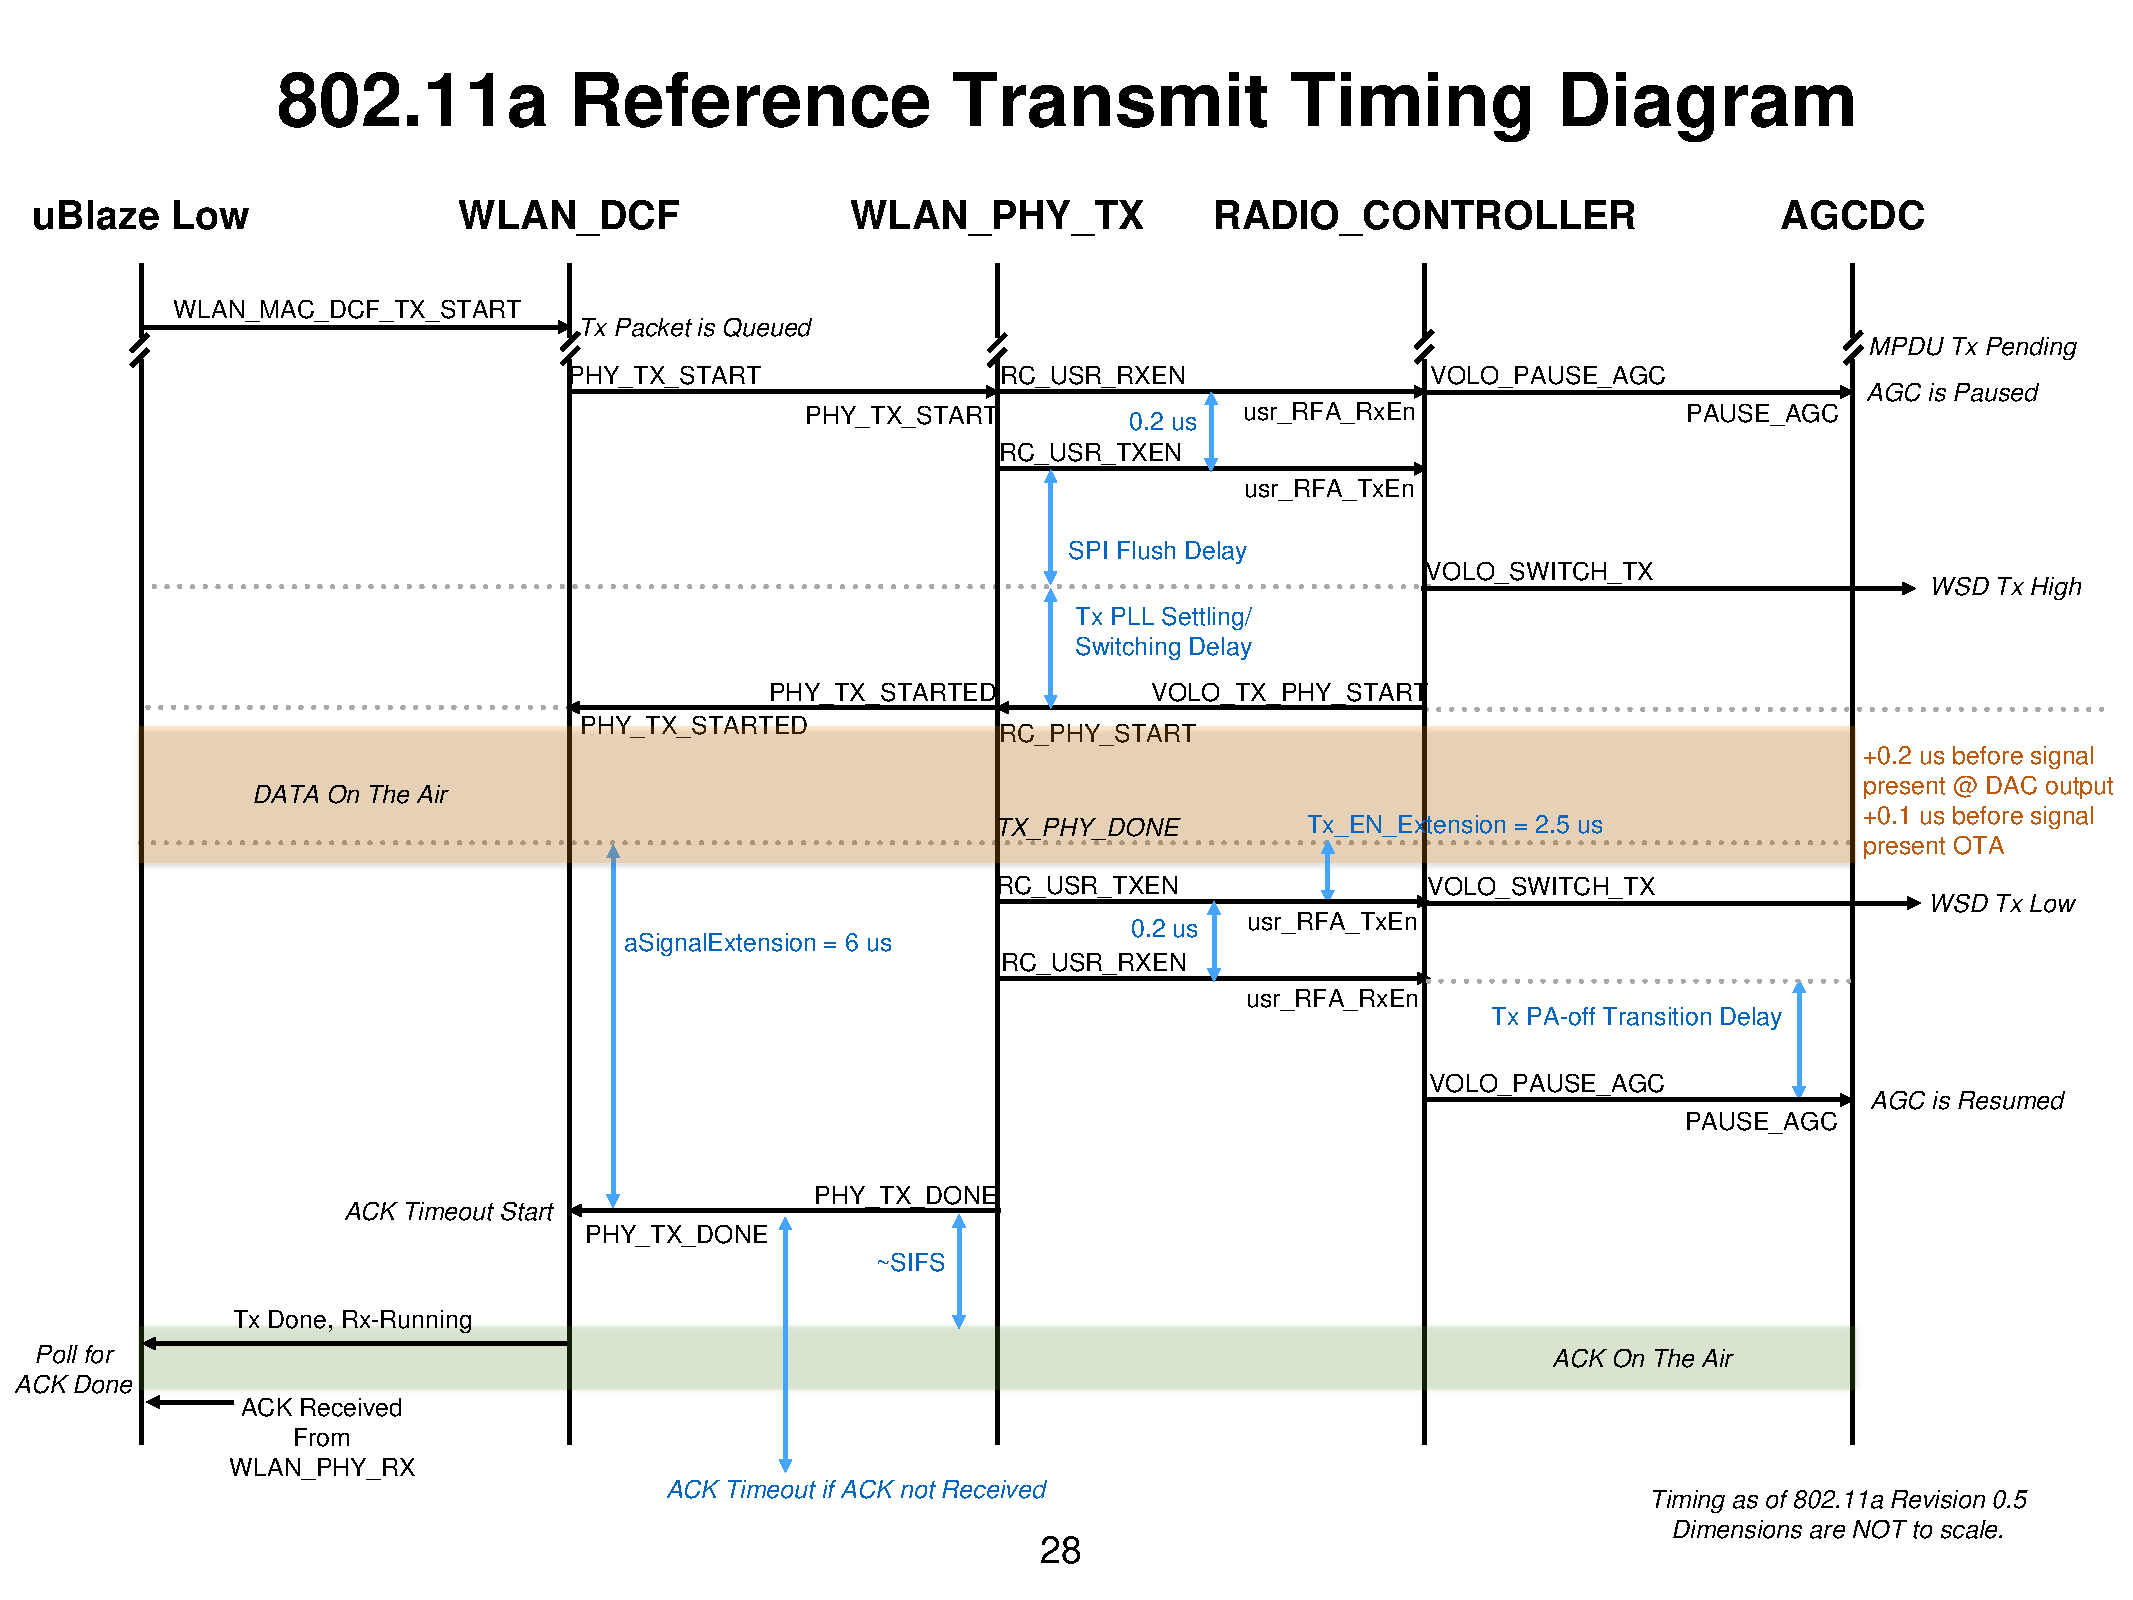
\includegraphics[width=0.9\linewidth]{figs/wurc/wurc_80211_timing_reference}   
    %\caption{Timing diagram for calibrating PHY hardware delays. \rgnote{TODO: write up this section regarding fast 802.11 Tx/Rx switching and its impact on performance} }
%\label{fig_wurc_timing}
%\end{figure}



%%###############################################
 \section{WURC Software Architecture}
\label{sec_wurc_sw_arch}

	As a software-defined radio system, the real-time software architecture of the \ac{WURC} platform represented a significant design challenge spanning high-level software architecture and low-level \ac{HDL} development.
	First, \ac{WURC} was designed as a modular, scalable system, and we desired to compartmentalize as many functions as possible while still retaining cross-layer access and control.
	Second, we wished to utilize existing \ac{PHY} prototyping frameworks such as WARPLab \cite{warplab} and the 802.11 Reference Design \cite{warp80211} from the \ac{WARP} project to provide starting points for implementing our \ac{MU-MIMO} testbed and 802.11af platform, respectively.

	To that effect, we designed a platform with an embedded micro-controller, the Texas Instruments Stellaris LM3S5R36 \cite{ti2012stellaris}, that would serve as a controller and abstraction layer for the agile software-defined radio transceiver, Lime Microsystems LMS6002D, and present high-level radio control functions to the host system.
	The software libraries embedded within the micro-controller were designed to be self-contained and portable, thus allowing a host system to integrate \ac{WURC} with minimal changes to the platform code, and to port this driver library to other hardware architectures easily.
	In this section, we present the software and firmware architectures for the WURC-based platformed presented in this thesis.

% WURC 802.11 Software/Firmware Architecture
\begin{figure}[p]
	\centering
  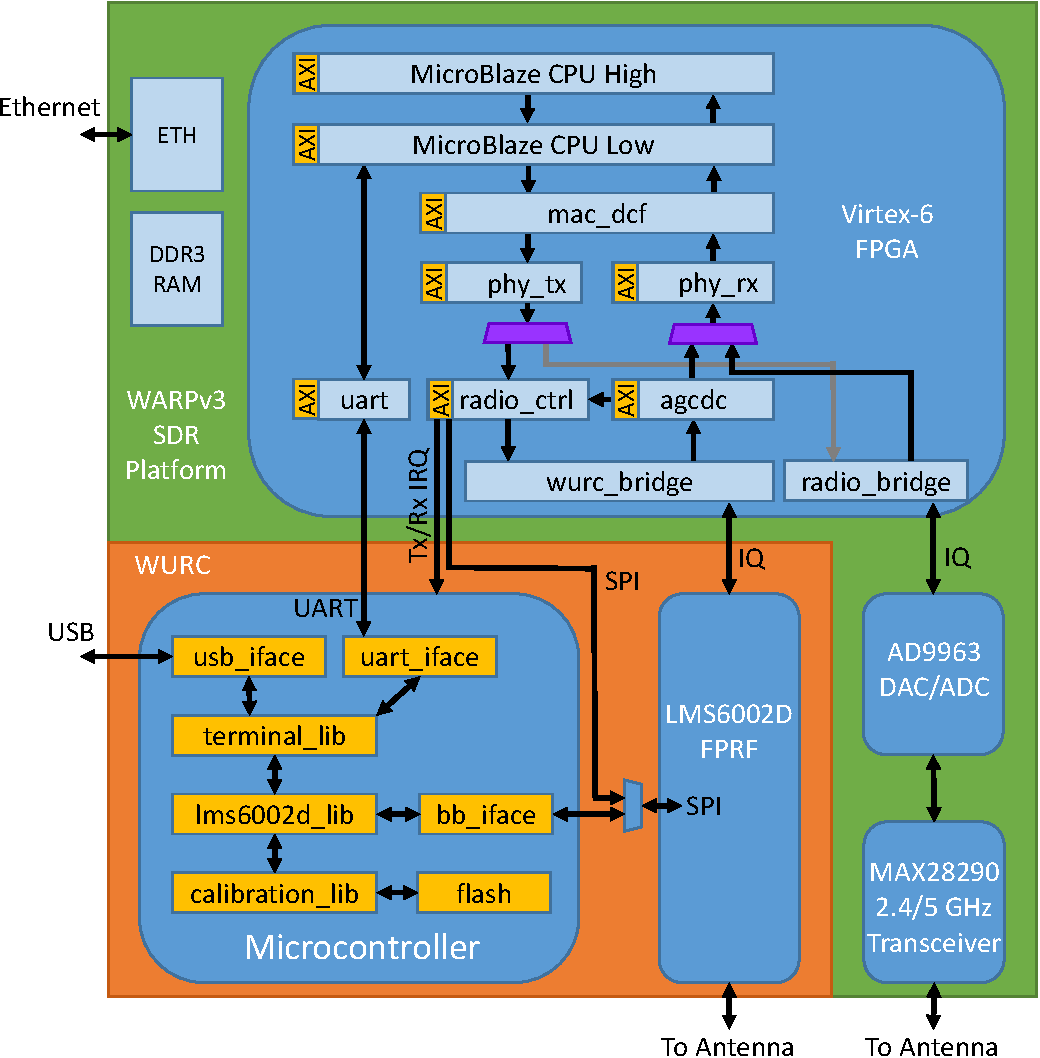
\includegraphics[width=1\linewidth]{figs/wurc/wurc_80211_hdl_design}   
  \caption{Software and HDL architecture of WURC/WARPv3 802.11 design.}
	\label{fig_wurc_80211_arch}
\end{figure}
	
% LMS6002D Library
\subsection{Agile \ac{SDR} Transceiver Driver \texttt{lms6002d\_lib}}
\label{sec_wurc_lms_lib}

	We designed and tested a platform-agnostic open-source C library of general calibration and configuration functions tailored for the LMS6002D agile RF transceiver \cite{guerra2013lms6002d}.
	The general architectural design and major interfaces between components is presented in Figure~\ref{fig_wurc_80211_arch}.
	The \ac{WARP} hardware components are contained within the green part of the system diagram while the \ac{WURC} hardware components are encapsulated within the red part (matching the color scheme in Figure~\ref{fig_warp_wurc_hw}; \ac{FPGA} code blocks for new \texttt{radio\_ctrl}, \texttt{agcdc}, and the \texttt{wurc\_bridge} modules were also developed.
	Aside from extremely time-sensitive operations such as receive gain control, all communications to the transceiver are filtered through a driver library \texttt{lms6002d\_lib} executing on a microcontroller embedded on each \ac{WURC} board.
	
	This encapsulation is necessary since the amount of parameter tuning, calibration, and self-test necessary to support basic analog transceiver functions grows significantly the more flexible a \ac{SDR} transceiver becomes.
	In application-specific radios, a discrete set of operational modes may be programmed and optimized; a truly agile transceiver must support a continuous range of center frequencies, modes of operation (TDD/FDD), channel bandwidths and analog waveforms, each requiring specific optimization.

	For example, changing the radio center frequency in an agile transceiver requires a complex set of actions: select the appropriate frequency synthesizer, tune synthesizer RC constants for optimal noise performance, load analog calibration values for IQ imbalance compensation, tune anti-aliasing filter RC constants, and calibrate analog component DC levels to remove \ac{LOFT} amongst other actions.
	As a result, many simple radio functions take hundreds of control register interactions with the underlying LMS6002D transceiver; we managed this complexity by encapsulating these actions with high-level functions designed to abstract the analog front-end and enumerated in Appendix~\ref{sec_wurc_console}.

	For large arrays of \ac{WURC} radios, a host can broadcast simple commands to initialize and configure the analog \ac{WURC} baseband via the \ac{UART}, and the on-board microcontrollers will compensate for the state and process variation for each radio while monitoring and reporting faults to the host system.
	
	This design offloaded a very significant amount of complexity and computation from the FPGA host and is one necessary component for scaling the number of radio modules in a large-scale \ac{WURC} array.

% LMS6002D Calibration
\subsubsection{SDR Transceiver Calibration \texttt{calibration\_lib}}
\label{sec_wurc_calibration}

	The calibration library is designed to interact with non-volatile flash memory on each \ac{WURC} device to store and retrieve radio calibration data generated for each \ac{WURC} during manufacturing.
	These analog compensation values are loaded in response to frequency and gain settings for the purpose of compensating for process variation in the LMS6002D direct-conversion transceiver.
		There are two types of analog radio calibration that are dependent on \ac{IC} manufacturing process variation and that we found were persistent for the lifetime of the LMS6002D transceiver.

	The first, \acf{LOFT}, is caused when the RF oscillator couples to the input of the receive mixer such that it mixes with itself down to baseband and appears as a strong tone at the 0th frequency, or DC component.
	This is a well-known impairment that is intrinsic to direct-conversion transceiver architectures and which can be compensated by applying a correction DC offset signal proportional to the strength of the receive \ac{LOFT}.
	We have found this value to be consistent, frequency-dependent, and smooth across the UHF band using \ac{WURC} hardware, therefore we store a series of scalar DC analog voltage correction levels in non-volatile flash memory that are loaded into correction DACs embedded in the LMS6002D receive chain each time the receive frequency is tuned by the driver.
	The goal of the compensation signal is to counter-act the known \ac{LOFT} DC component such that the finite \ac{ADC} dynamic range is not exceeded.
	Once a compensation signal is added to the analog signal, the remaining \ac{LOFT} DC component can be easily removed in the digital domain with a digital low-pass filter.

	The second calibration is for IQ imbalance, which is caused by differences between the I and Q circuit paths within the LMS6002D quadrature transceiver in terms of gain and phase.
	These imbalances result in the generation of image tones on both the input and output signals after quadrature mixing \cite{tubbax2005compensation}.
	Similar to \ac{LOFT}, this impairment is consistent, frequency-dependent, and smooth across the UHF band.
	However, given the digital architecture of our system, these corrections must be applied in the digital domain on the FPGA and are therefore more complex to implement\footnote{Recent generations of agile RF transceivers include these digital correction block on-chip \cite{lime2018lms7002M, adi2018adrv9009}}.
	We calculate optimal phase and magnitude compensation values during manufacture for each 6~MHz UHF channel, then store a triplet of pre-computed coefficients in non-volatile flash memory that will perform the needed vector rotation and gain adjustment on the digital IQ stream.
	These values are loaded to the respective transmit or receive data flow each time the frequency is changed via the UART terminal interface to the host logic.
	
	Since we find the correction values to be smooth functions,\footnote{In fact, a sure indicator of a damaged or malfunctioning \ac{WURC} transceiver is non-smooth calibration coefficients with respect to frequency.} we are able to conserve non-volatile memory space by storing calibration values at several discrete points across our operating frequency range and interpolating calibration values for any arbitrary center frequency between calibration points.
	

% Discussion of the Terminal Interface
\subsubsection{WURC User Control Interface \texttt{terminal\_lib}}
\label{sec_wurc_terminal}

	In order to make the architecture portable and extensible, we separated I/O functions with the \ac{FPRF} transceiver into a separate \texttt{bb\_iface} \ac{API} and user \acp{API} into a custom terminal (\texttt{terminal\_lib}) with the ability to interact through multiple, abstracted character-based interfaces like \ac{USB} (\texttt{usb\_iface}) or \ac{UART} (\texttt{uart\_iface}).
	This makes our designed driver libraries useful for other systems based on the LMS6002D \ac{IC} and readily portable to other CPU architectures.

	The available top-level console commands are described in Appendix~\ref{sec_wurc_console} and can be accessed at any time from either a user connected to the \ac{WURC} terminal directly via \ac{USB}, or from the host via the WARP terminal.

% Tx/Rx Optimization
\subsubsection{Transmit/Receive Switching IRQ Abstraction}
\label{sec_txrx_switching}

For \ac{TDD} protocols like 802.11af, the hardware switching time to turn a radio from transmit to receive or vice-verse is one of the fundamental parameters that drives protocol timing and can be as low as 10~$\mu$s \cite{std11af}.

	This seemingly simple operation encapsulates a number of sequential operations to disable the previously active RF chain and enable the previously inactive chain; on an agile \ac{SDR}, the precise timing of that sequence becomes necessary to manage carefully.
	To this effect, we designed the \ac{WURC} to present a single I/O pin to the host hardware that could be switched high or low while the \ac{WURC} is configured for \ac{TDD} mode to signal the module to shift into transmit or receive mode, respectively.
	Similar to the fast analog gain control design presented in Section~\ref{wurc_agc}, careful analysis and optimization of sequence timing is important to meet timing deadlines.

	We designed the single-pin abstraction to provide a simple Tx/Rx interface to the host that would trigger an interrupt-driven subroutine within the Stellaris microcontroller.
	Figure~\ref{fig_wurc_80211_arch} shows the ``Tx/RX IRQ'' line directly connecting the radio controller to a Stellaris interrupt pin.
	In order to meet timing requirements, it was necessary to flatten the interrupt functional structure and hand-optimize serial command writes and GPIO signals in assembly code in order to enable/disable amplifiers in a precisely timed sequence.
	Combined with tuning of the \ac{WURC} amplifier noise-immunity RC constants and the LMS6002D's frequency synthesizer settling times, we were able to achieve a Tx/Rx turnaround time less than 5~$\mu$s, providing sufficient margin for the MAC layer to make decisions.
	
	%This same logical interface, allowing a host to simplify Tx/Rx switching while pushing real-time control of radio hardware to separate embedded logic, is a key design concept in more recent \acp{SDR} platforms.


%% Discussion of the 802.11 Integration 
%\subsection{WARP 802.11 Integration}
%\label{sec_wurc_80211}
%
	%We integrated the \ac{WURC} \ac{SDR} radio platform with the WARP platform as shown in Figure~\ref{fig_wurc_80211_arch}.
%\rgnote{I couldn't think of anything not engineering to put here. So cut.}

% Discussion of the WARPLab Integration
\subsection{WARPLab Integration}
\label{sec_warplab}

	The WARPLab framework from Mango Communications is an open-source experimental framework that enables a host to synchronize an arbitrarily large number of WARPv3 hosts connected via a Layer 3 backhaul network to perform non-realtime over-the-air experiments \cite{warplab} using MATLAB as a signal processing and coordination environment.
	When a subset of those WARPv3 radios physically share their RF reference clocks and timing reference triggers, the over-the-air transmissions can be made coherent.
	
	WARPLab operates by utilizing MATLAB scripts to generate transmit sample buffers for arbitrary topologies of coherent radio arrays and individual radio nodes with arbitrary baseband signals.
	Once pre-loaded across the experimental topology, a synchronized and hardware-accelerated ethernet trigger\footnote{Handling of the received ethernet trigger on WARPv3 node is performed in \ac{FPGA} hardware, avoiding non-deterministic network stack processing latency.} packet is sent to all nodes, causing them all to simultaneously transmit and/or receive on their radios as pre-configured.
	The receive waveforms are stored in a local receive sample buffer for retrieval.
	A layer 2 communications framework built on MATLAB allows rapid distribution of transmit samples buffers and retrieval of receive sample buffers for post-processing. 
	Of particular importance for enabling conherent \ac{MIMO} transmissions, an array of coherent WARPv3 nodes sharing an RF reference clock does not simply use the ethernet trigger packet for timing synchronization as that would introduce non-deterministic transport delays between nodes.
	Rather, they designate a master node that distributes a simultaneous \ac{GPIO} trigger signal to all slave WARPv3 nodes in order to ensure sample-level synchronization of the coherent radios.
	More details are provided within the WARP project documentation \cite{warplab}.
	
	In Appendix~\ref{sec_warplab_arch}, we present a mapping of WARPLab's functional architecture and highlight parts of the MATLAB code base where we were able to extend WARPLab functionality to transparently support \ac{WURC} transceivers in addition to the built-in WARPv3 transceivers.
	This enabled WARPLab-based experiments to be performed in \ac{TVWS} bands.
	
% WARPLab timing analysis
\subsubsection{WARPLab Latency Analysis}
\label{sec_warplab_timing}

	WARPLab 7 contains a number of transport improvements that result in the ability to perform near-real-time experiments by rapidly performing cycles of: precompute, load, transmit/receive, fetch, and process on the order of 2.5~ms.
	A fast central coordinator using jumbo ethernet frames for transporting IQ buffers and a compiled MATLAB-mex transport layer can operate at per-packet time intervals by decreasing both ethernet transport overhead and network stack latency.
	We observed that extra switches between WARPLab nodes produce measurable switching delay and recommend the use of long ethernet cables and minimization of the number of ethernet hops for WARPLab backhaul.

	While WARPLab is a powerful \ac{PHY} prototyping tool, the two largest drawbacks of WARPLab is that it: 1) requires a central coordinator connected via gigabit ethernet switches; and 2) real-time protocol implementations generally require processing at microsecond symbol-level timescales whereas WARPLab performs centralized signal processing on millisecond packet-level timescales.
	These two factors hinder long-distance or mobile experiments where the installation of a wired ethernet backhaul is quite difficult or nodes move too rapidly to make protocol decisions using WARPLab's centralized framework.
	
	%\rgnote{Put the WARPLab 4x1 HDL architecture diagram here}
	
%\subsubsection{WARPLab Example Application: Spectrum Scanner}
%\label{sec_scanner_app}
%
%
%
%\begin{figure}[p]
	%\centering
  %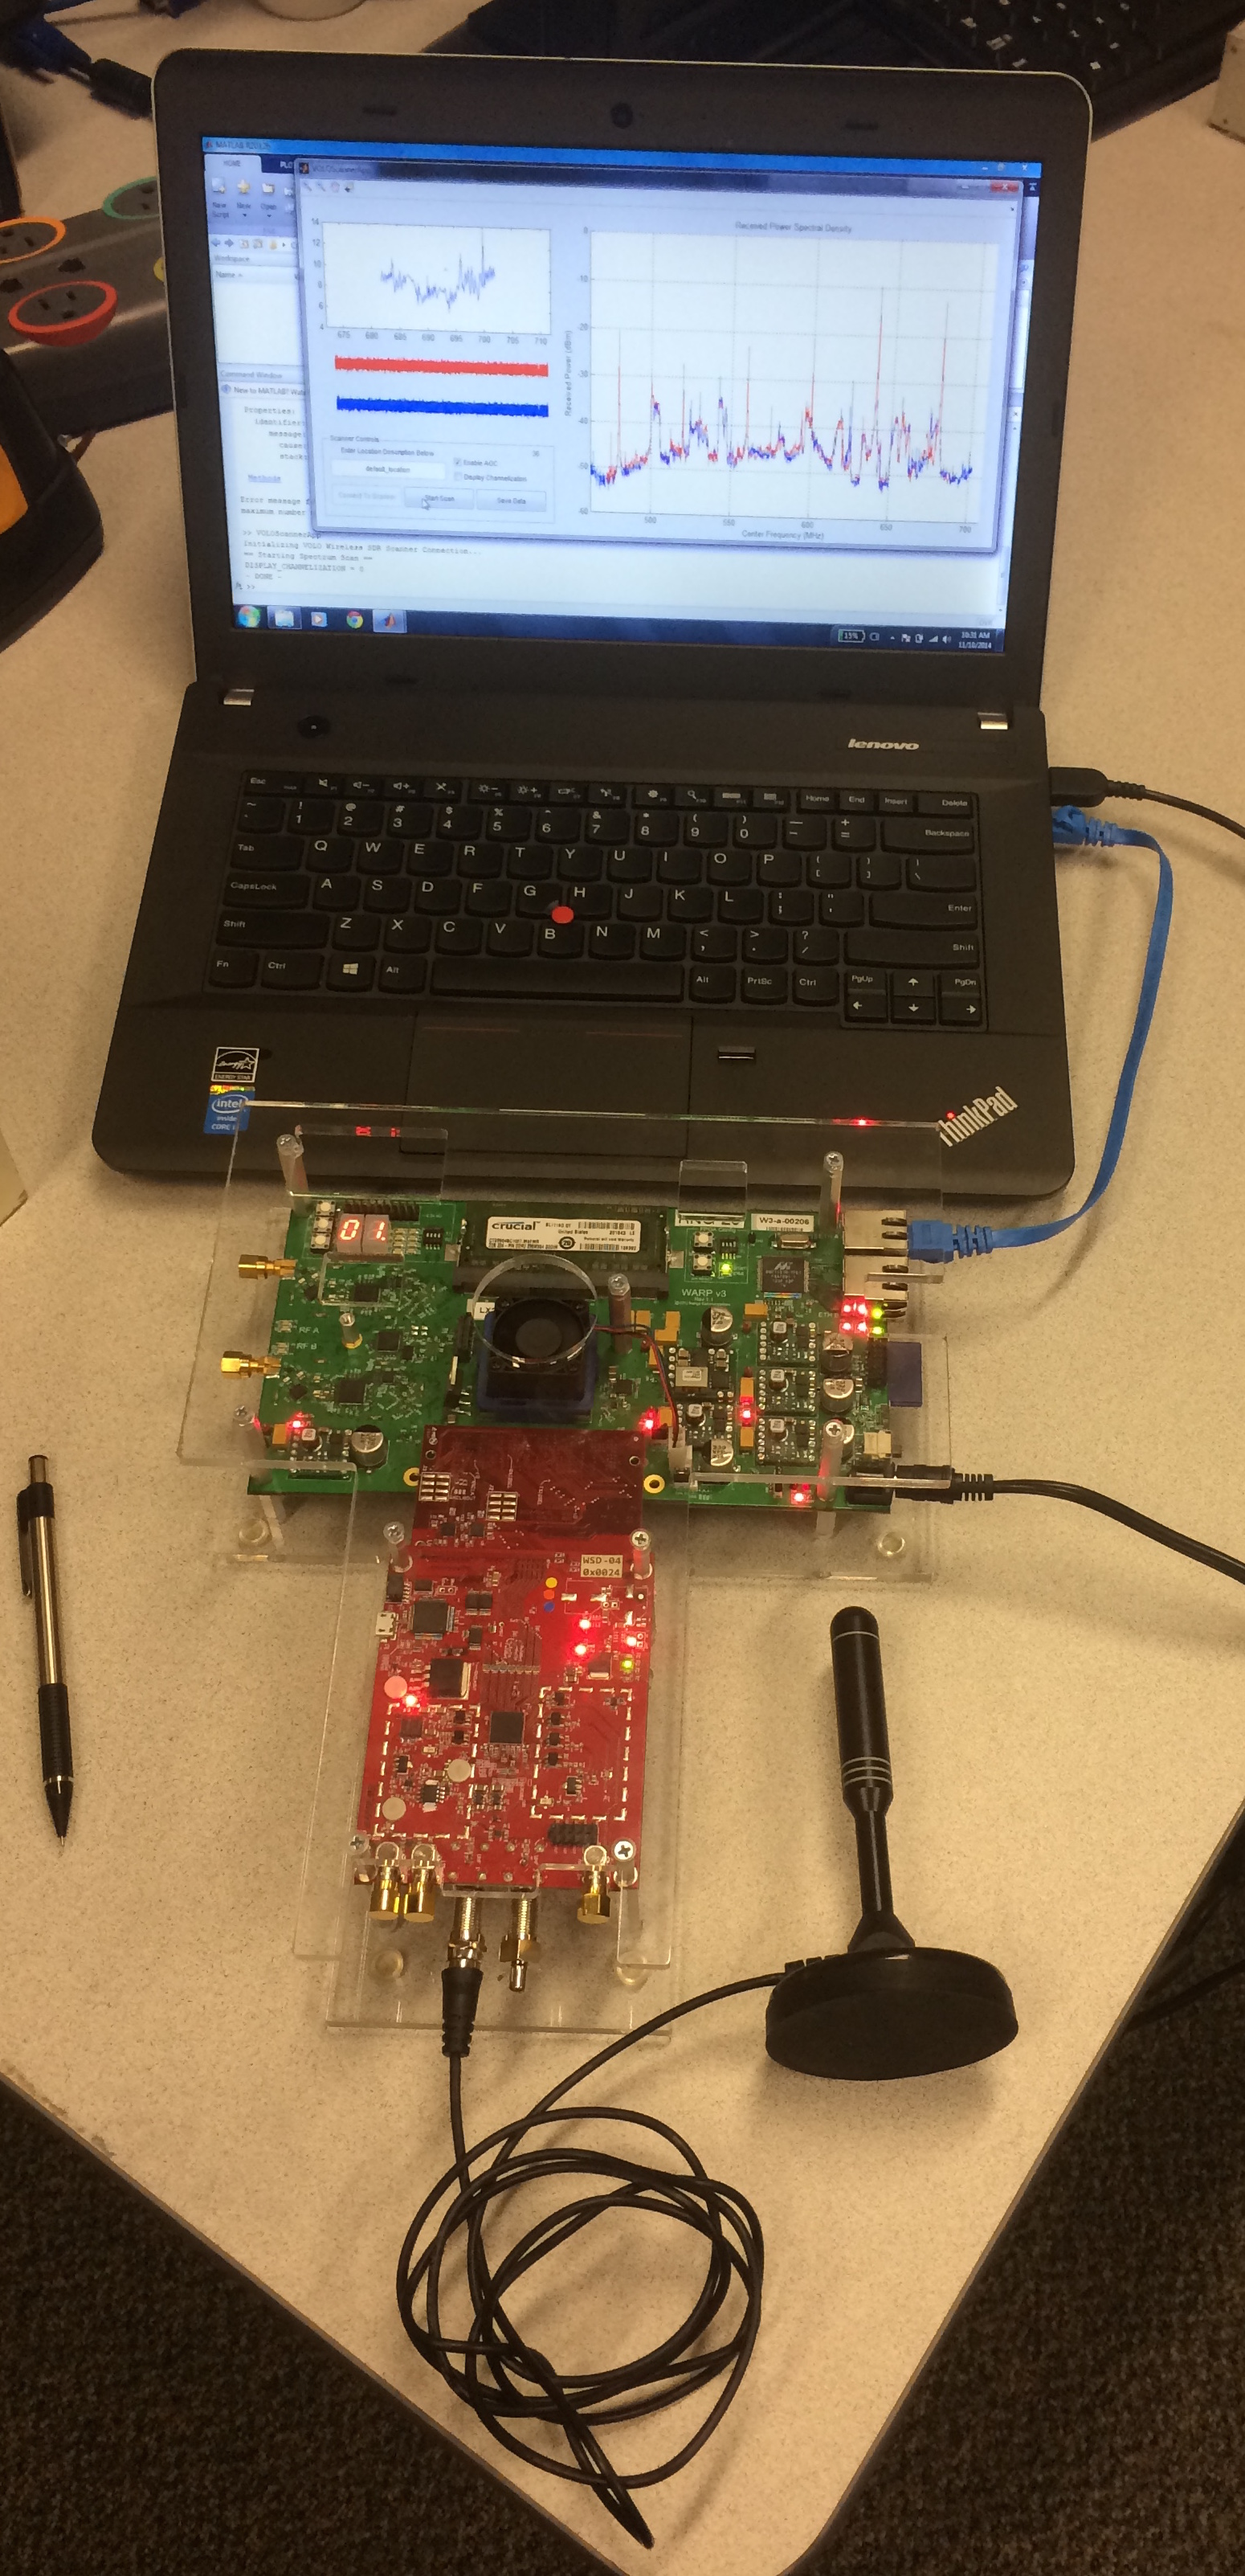
\includegraphics[width=0.4\linewidth]{figs/wurc/scanner_hw}   
  %\caption{Hardware setup for WURC Spectrum Scanner application.}
	%\label{fig_wurc_scanner_hw}
%\end{figure}
%
%\begin{figure}[p]
	%\centering
  %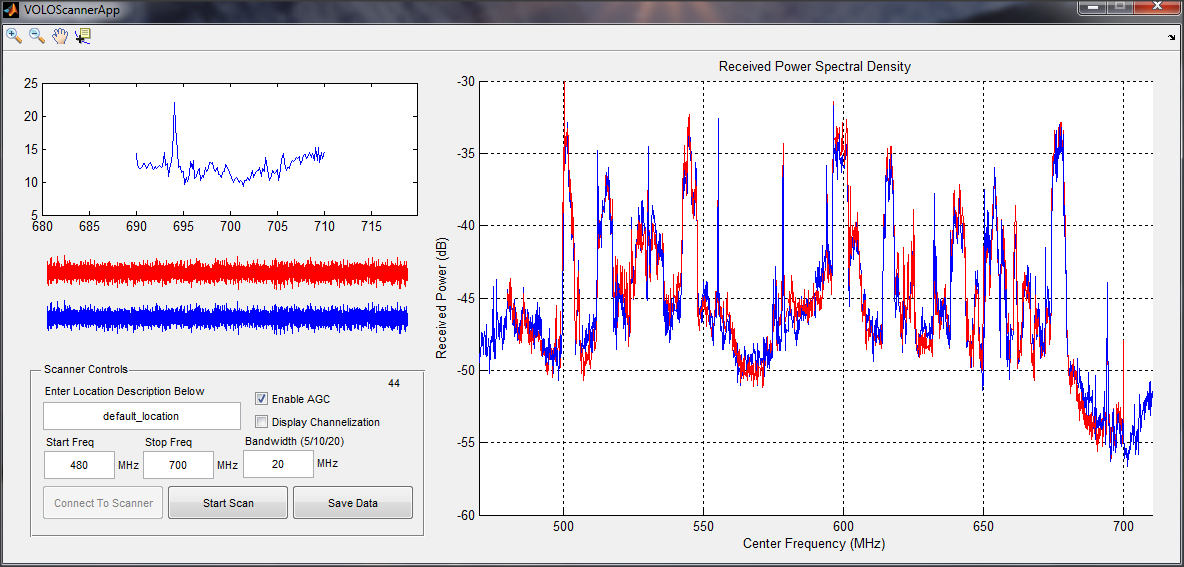
\includegraphics[width=0.8\linewidth]{figs/wurc/scanner_run_indoor}   
  %\caption{GUI for WURC Spectrum Scanner application.}
	%\label{fig_wurc_scanner_gui}
%\end{figure}


